\section{System Overview}\label{sec:system-overview}
\subsection{Full Gesture Recognition System}\label{subsec:full-gesture-recognition-system}
This research focuses on finding an appropriate neural network architecture to perform gesture recognition on a microcontroller, but it is only part of a larger project to create an entire gesture recognition system.
This project is composed of the following tasks:
\begin{enumerate}
    \item Optimizing the number and placement of OPT101 photo diodes.
    \item Reading, processing, and sanitizing data from photo diodes.
    \item Creating an appropriate dataset for training a neural network to recognize gestures.
    \item Finding an appropriate neural network architecture on the created dataset and ensuring gestures can be recognized in real-time on an Arduino Nano 33 BLE\@.
\end{enumerate}

The research presented in this paper aims to complete task 4.
Although tasks 1--3 were completed by other group members and are beyond the scope of this research, they are worth mentioning to provide some context regarding the rest of the gesture recognition system.
Due to the findings from these tasks, the final system uses 3 photodiodes and can recognize 8 different gestures, while each gesture is composed of 100 readings from each photodiode.
This is relevant for task 4, as it means that whatever neural network is implemented must use a 2D array of size 3 by 100 (split into \textit{n} frames after 3D-formatting) as an input feature and be able to distinguish between 8 output classes, as illustrated in figure~\ref{fig:system}.

\begin{figure}[h]
    \centering
    \captionsetup{justification=centering}
    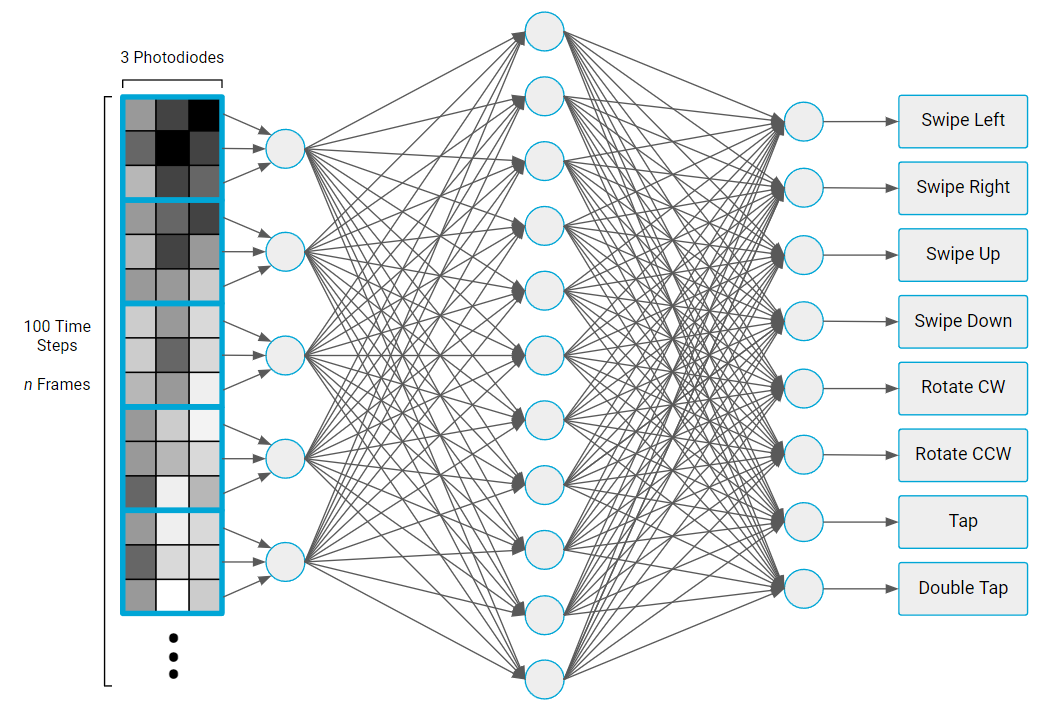
\includegraphics[width=\linewidth]{figures/system_advanced}
    \caption{Visualization of the inputs \& outputs for a generic neural network in the gesture recognition system.}
    \label{fig:system}
\end{figure}

\subsection{Dataset}\label{subsec:dataset}
Having a varied, expansive, and representative dataset is crucial for training a machine learning with high real-world accuracy.
Fortunately, the task of creating such a dataset for recognizing gestures using photodiode data was done by another member of the project group.
This dataset is contains 5 repetitions of each of the 8 gestures per hand across 50 participants, leading to 4000 total data instances.
Although the dataset contains instances from a variety of environments and lighting setups, these are mostly indoor locations as this is the planned use case for the system.
The dataset was also mostly recorded on the TU Delft campus, meaning the demographic of participants is somewhat skewed.
Most notably, the dataset contains substantially more instances of males compared to females, and more right-handed participants than left-handed.
However, this is not expected to have a large impact on the final model performance.